\section{Problem 1}
\subsection{(a)}
Assessing the following:
$$\theta_n = \frac{n}{\sum_{i=1}^{n} x_i}$$

I'm working with a geometric distribution so I have the following PMF:
$$ P_\theta(x) = (1 - \theta)^{x-1} \theta $$

rewriting the expression using pi-notation (Product notation):
$$ P_\theta (X_i = x_i) = P_\theta(x_i) = (1 - \theta)^{x_i - 1} \theta $$
$$ P_\theta (x_1, ..., x_n ; \theta) = \prod_{i=1}^{n} (1 - \theta)^{x_i - 1} \theta $$

Rewriting this new expression by taking the logarithm of the expression:
\begin{align*}
    & log(\prod_{i=1}^{n} (1 - \theta)^{x_i - 1} \theta) = \sum_{i = 1}^{n} (log ( (1 - \theta)^{x_i - 1} + log(\theta) )) \\
    & = l(\theta) = \sum_{i = 1}^{n} (x_i - 1) log(1 - \theta) + log(\theta)
\end{align*}

Differentiating the expression and setting it equal to zero and dividing the expression into three sums
\begin{align*}
    & \frac{\partial l}{\partial \theta} = \sum_{i = 1}^{n} ( (x_i - 1) (-1) \frac{1}{1 - \theta} \frac{1}{\theta} ) = 0 \\
    & \\
    & \Longrightarrow \sum_{i = 1}^{n} ( (\frac{-1}{1 - \theta} + 1 \frac{1}{1 - \theta}) + \frac{1}{\theta}) = 0 \\
    & \\
    & \frac{-1}{1 - \theta} \sum_{i = 1}^{n} x_i + \sum_{i = 1}^{n} \frac{1}{1 - \theta} + \sum_{i = 1}^{n} \frac{1}{\theta} = 0 \\
    & \\
    & \Longrightarrow \frac{-1}{1 - \theta} \sum_{i = 1}^{n} x_i + n \frac{1}{1 - \theta} + n \frac{1}{\theta} = 0
\end{align*}

multiplying with $ (1 - \theta) $ through the equation:

\begin{align*}
    & - \sum_{i = 1}^{n} x_i + n + \frac{n}{\theta}(1 - \theta) = 0 \\
    & \\
    & - \sum_{i = 1}^{n} x_i + \frac{n \theta + n(1 - \theta)}{\theta} = 0 \\
    & \\
    & - \sum_{i = 1}^{n} x_i + \frac{n}{\theta} = 0 \\
    & \\
    & \Longleftrightarrow \frac{n}{\theta} = \sum_{i = 1}^{n} x_i \Longrightarrow \theta = \frac{n}{\sum_{i = 1}^{n} x_i}
\end{align*}

Calculating the second derivative of the function, in order to check if the function is
either convex or concave. Which tells whether it's a maximum or minimum I've found.
\begin{align*}
    & \frac{\partial^2 l}{\partial \theta \partial \theta} = \frac{-1}{1 - \theta} \sum_{i = 1}^{n} x_i + n \frac{1}{1 - \theta} + n \frac{1}{\theta} \\
    & \\
    & = - (-1)\frac{-1}{(1 - \theta)^2} \sum_{i = 1}^{n} x_i + n (-1) \frac{-1}{(1 - \theta)^2} + n (-1) \frac{-1}{\theta^2} \\
    & \\
    & = \frac{-1}{(1 - \theta)^2} \sum_{i = 1}^{n} x_i + n \frac{1}{(1 - \theta)^2} - n \frac{1}{\theta^2} \\
    & \\
    & = - \frac{\sum_{i = 1}^{n} x_i}{(1 - \theta)^2} + \frac{n}{(1 - \theta)^2} - \frac{n}{\theta^2} \\
\end{align*}
Thus since the function will always be negative, I can conclude that I'm dealing with a maximum
\begin{align*}
    & \sum_{i = 1}^{n} x_i \geq n \quad \text{since} \quad x_i \exists Z_+
\end{align*}
Which concludes the proof.

% \begin{minted}[linenos, bgcolor = bg]{python}

% \end{minted}


% \begin{figure}[H]
%     \centering
%     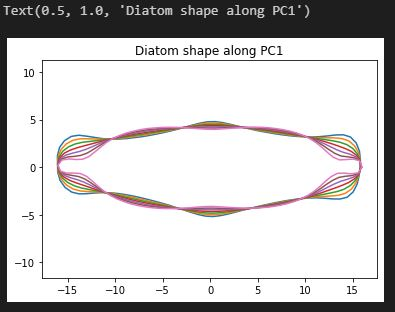
\includegraphics[width=0.75\textwidth]{Figures/Result_of_diatoms.JPG}
%     \caption{Plotted diatom}
% \end{figure}

